\section{Platform \& Business Applications}\label{sec:02}  

  The notion of the ``platform'' and ``platform-oriented'' software development is nowadays well accepted and in most cases is understood more generically than a capability to operate in a specific operating system.
  Usually, ``platform'' is understood as an execution environment and a set of technologies used for developing software applications for a certain domain.
  Any software application can be based on several platforms, which can be visualised as layers placed on top of each other with an actual application at the very top.
  What is defining for any platform is its unique model that isolates software developers from the details of lower level technologies and platforms.

  \begin{wrapfigure}{r}{55mm}
    \centering    
    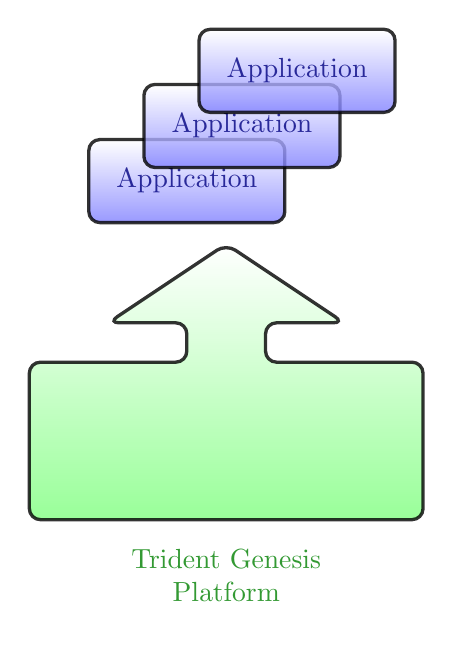
\begin{tikzpicture}[node distance=1cm, auto, opacity=0.8]
      \tikzset{
	  mynode/.style={rectangle,rounded corners,draw=black, top color=white, bottom color=blue!50,very thick, inner sep=1em, minimum size=3em, text centered, text=blue!50!black},
	  platform/.style={rectangle,rounded corners,draw=black, top color=white, bottom color=green!50!white,very thick, inner sep=1em, minimum size=3em, text centered, text=green!50!black}
      }  
      \node at (1, 1) [mynode] (ap1) {Application};
      \node at (1.7, 1.7) [mynode] (ap1) {Application};
      \node at (2.4, 2.4) [mynode] (ap1) {Application};

      \def\platformpath{-- +(5cm,0cm) -- +(5cm,2cm) -- +(3cm,2cm) -- +(3cm,2.5cm) -- +(4cm,2.5cm) -- +(2.5cm,3.5cm) -- +(1cm,2.5cm) -- +(2cm,2.5cm) -- +(2cm,2cm) -- +(0cm,2cm) -- cycle}
      \draw (-1,-3.3) [platform] \platformpath 
	    node [below,text width=7em, text centered,xshift=2.5cm] {Trident Genesis Platform};  
    \end{tikzpicture} 
  \end{wrapfigure}
  
  From this perspective Trident Genesis is not different providing a necessary abstraction for using lower level technologies without changing the source code of a business application.
  For example, it provides the developers with its own model for working with data, which abstracts out the specifics of a particular database, which allows using different databases without modifying the business application source code.
  This way a small-scale application can happily use H2 or MySQL, while a large-scale application would work with Oracle Database or MS SQL Server.

  At the very beginning the TG platform was targeted at inhouse purposes for migrating existing and developing new business applications.
  Such practical-driven approach allowed capturing the existing experience building business application in a way that made TG not just a set of reusable components and libraries, but a complete application platform covering every aspect of the development and deployment application life-cycle.
  This in turn positioned TG as a standalone product, which does not mix in any specifics of a particular business application providing a generic way for building diverse business-oriented information systems.

  The TG platform provides well thought out set of feature sufficient for providing solutions to a large variety of business tasks/problems.
  This results in reliable and controlled interoperability between underlying technologies governed by the platform without the need for introducing external dependencies resulting in ``stitches'', which often become the cause of many software defects.
  An excellent example of such interoperability is the developed \emph{type system}.
  When building applications on top of TG, developers use the provided systems of types for interacting with web-resources, databases and for implementing business logic as well as the user interface.
  This removes the need for developers to work on type transformations when implementing different layers of the information system.
  
  As has been outlined earlier, the majority of software applications are not created from scratch, but enhanced and modified as business demands.
  Especially for business applications it is critical to have the ability for their efficient customisation by developers not involved in the original development of the system.
  This situation defines a special requirement for such systems to be easily comprehended, which has been taken into account when designing the TG platform.
  Building applications on top of TG provides a clear separation between technical and business aspects of software applications catering for their much higher level of customisability in order to meet customers' requirements.